\part{Parametry kamene \textit{viva12}}
\label{sec: parametryVIVA12}

Šatonová růže má 14 rovinných faset. Fasety označujeme zkratkami TOP, BOT a\\ UF1~-~UF12, kde

\begin{tabular}{L{2cm} l}
TOP & $-$ tabulka,\\
BOT & $-$ spodek,\\
UF1-UF12 & $-$ 12 bočních faset.\\
\end{tabular}\\

Označené fasety máme na obrázku \ref{fig:viva12Params} spolu s vyznačenými parametry

\begin{tabular}{L{2cm} l}
$d_{TOP}$ &$-$ průměr tabulky,\\
$d_{BOT}$ &$-$ průměr spodku,\\
$h$ &$-$ výška kamene,\\
$h_{RF}$ & $-$ výška lemu. 
\end{tabular}\\
 
Poznamenejme, že lem modelujeme množstvím faset, které po spojení aproximují oválný tvar. Tyto fasety mají v simulaci absorpční charakter. Světelné svazky, které dopadnou na lem, zaniknou.   

\begin{figure}[htps]
\centering
\begin{minipage}[c]{0.4\textwidth}
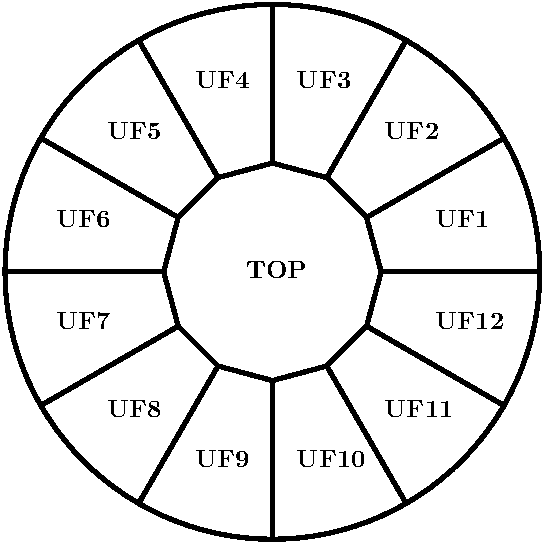
\includegraphics[width=\textwidth]{vivi12Facets1.pdf}
\end{minipage}
\begin{minipage}[c]{0.56\textwidth}
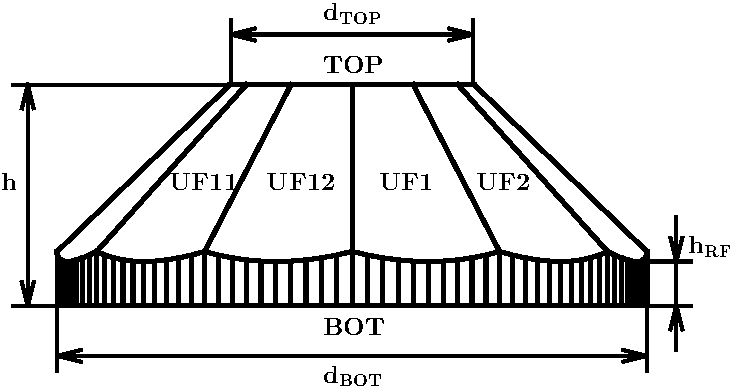
\includegraphics[width=\textwidth]{vivi12Facets2.pdf}
\end{minipage}
\caption{Šatonová růže s označenými fasetami a parametry. Pohled shora je zobrazen vlevo, bokorys vpravo.}
\label{fig:viva12Params}
\end{figure}



\clearpage




